\documentclass[11pt,a4paper]{article}
\usepackage[utf8]{inputenc}
\usepackage[T1]{fontenc}
\usepackage{amsfonts}
\usepackage[french]{babel}
\frenchbsetup{StandardLists=true} % à inclure si on utilise \usepackage[francais]{babel}
\usepackage{enumitem}
\usepackage{amssymb}
\def\nbR{\ensuremath{\mathrm{I\! R}}}
\usepackage{amsmath}
\DeclareMathOperator{\e}{e}

\usepackage[left=2cm,right=2cm,top=2cm,bottom=2cm]{geometry}
\usepackage{multirow}
\usepackage[dvipsnames]{xcolor}
\usepackage{parskip}
\usepackage{caption}

\usepackage{circuitikz}



\usepackage[T1]{fontenc}
\usepackage{fouriernc}

\usepackage{graphicx}
\usepackage{setspace}
\singlespacing

\usepackage{tcolorbox}
\usepackage{framed}
\usepackage{multicol}

\usepackage{fancybox}
\usepackage{fancyhdr}
\pagestyle{fancy}
\renewcommand\headrulewidth{1pt}
\fancyhead[L]{Lycée Denis Diderot }
\fancyhead[R]{Classe de Première Bac Pro}
\setcounter{page}{3}\fancyfoot[C]{page \thepage}
\fancyfoot[R]{Année 2025-2026}
\fancyfoot[L]{Alexis RUIZ}
\usepackage{pstricks,pst-plot}
\usepackage{tikz}
\usepackage{tkz-tab}
\usetikzlibrary{arrows}
\usepackage{pifont}

\newcommand{\ud}{\mathrm{d}}
\newcommand{\V}{\overrightarrow}
\newcommand{\Rep}{(O;\V{u};\V{v})} 
\newcommand{\cadreblanc}[1]{%
\medskip\framebox[\linewidth][c]{%
\rule{0mm}{#1mm}}\par
\medskip}
\setlength{\columnseprule}{.25mm}
\usepackage{multirow,tabularx,booktabs}
\usepackage{colortbl}
\usepackage{wrapfig}

\usepackage{qrcode}
\usepackage[tikz]{bclogo} 
\usepackage{ProfCollege}
\usepackage{pgfplots,mathtools}
\usepackage{bclogo}

\newcommand{\cadre}[1]
{
\vspace{2mm}
\begin{bclogo}[couleur = white,logo=,  arrondi = 0.3,barre=none]
{%
\rule{0mm}{#1mm}}\par
\medskip
\end{bclogo}}



\begin{document}
\newtcolorbox{mybox}{colback=blue!10!white,
colframe=black!5!black}

\newtcolorbox{mybox1}{colback=white,
colframe=black!5!black}

\begin{mybox1}
NOM : \hfill Prénom : \hfill ~~
\end{mybox1}

\vfill
\begin{mybox}
\begin{center}

\textbf{
\Large 
Contrôle 1 - Mesures du courant
}
\end{center}
\end{mybox}

\vfill 

\begin{mybox1}
Exercice 1 : Convertir (avec 1A = 1000 mA) ~ \hfill ~~ 1,5 pts
\end{mybox1}

\vspace{3mm}

\begin{multicols}{3}
$1200$mA = \dotfill A 
\vspace{5mm}

$800$mA = \dotfill A 
\vspace{5mm}

$21380$mA = \dotfill A 
\vspace{5mm}

$1,01$A = \dotfill mA
\vspace{5mm}

$10,81$A = \dotfill mA
\vspace{5mm}

$0,801$A = \dotfill mA
\vspace{5mm}
    
\end{multicols}


\begin{mybox1}
    Exercice 2 : Application de la loi des noeuds ~ \hfill ~~ 3,5 pts
\end{mybox1}




\begin{enumerate}
\item Indiquer à l'aide de flèches le sens du courant dans chaque branche.








\begin{center}
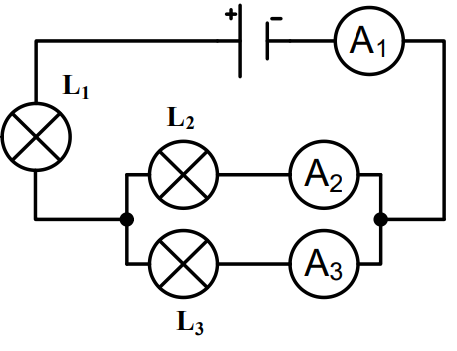
\includegraphics[scale=0.4]{images/exercice 3.png}
\end{center}
\item Soit $\mathrm{I_1 }$
l’intensité du courant dans la branche principale, $\mathrm{I_2 }$ dans la branche de $\mathrm{L_2}$ et $\mathrm{I_3 }$ intensité du
courant dans dans la branche de $\mathrm{L_3}$. \\[5mm]
Écrire la loi des noeuds.~~\dotfill 


\item On donne $\mathrm{I_2 }$ = 1,45 A et $\mathrm{I_3 }$ = 550 mA. Calculer $\mathrm{I_1 }$ \\

\dotfill 


\item  La lampe $\mathrm{L_3 }$ grille. L'ampèremètre $\mathrm{A_2 }$ mesure alors $\mathrm{I_2 }$ = 2 A. 
Que mesurera l'ampèremètre $\mathrm{A_3 }$ ? \\

\dotfill 

\item  Que mesurera l'ampèremètre $\mathrm{A_1 }$ si la lampe $\mathrm{L_3}$ est toujours grillée ? \\

\dotfill 
\end{enumerate}


\vfill 
\begin{mybox}
    ENIGME BONUS (+1)
    
\end{mybox}
Voici une suite logique de nombres : 6 ; 4 ; 8 ; 5 ; 15 … Quels sont les deux nombres suivants ?
\cadre{10}

\vfill






\end{document}